%!TEX root = ../TAMUTemplate.tex
%%%%%%%%%%%%%%%%%%%%%%%%%%%%%%%%%%%%%%%%%%%%%%%%%%%
%
%  New template code for TAMU Theses and Dissertations starting Fall 2016.
%
%  Author: Sean Zachary Roberson
%	 Version 3.16.09
%  Last updated 9/12/2016
%
%%%%%%%%%%%%%%%%%%%%%%%%%%%%%%%%%%%%%%%%%%%%%%%%%%%
%%%%%%%%%%%%%%%%%%%%%%%%%%%%%%%%%%%%%%%%%%%%%%%%%%%%%%%%%%%%%%%%%%%%%%
%%                           SECTION V
%%%%%%%%%%%%%%%%%%%%%%%%%%%%%%%%%%%%%%%%%%%%%%%%%%%%%%%%%%%%%%%%%%%%%



\section{Limits and Results}
\subsection{Event Yields}
\subsection{Impact of Systematic Uncertainties}
\subsection{Limits}

\begin{comment}
begin{figure}[!hbt]
	\centering
	\begin{subfigure}[t]{0.46\textwidth}
		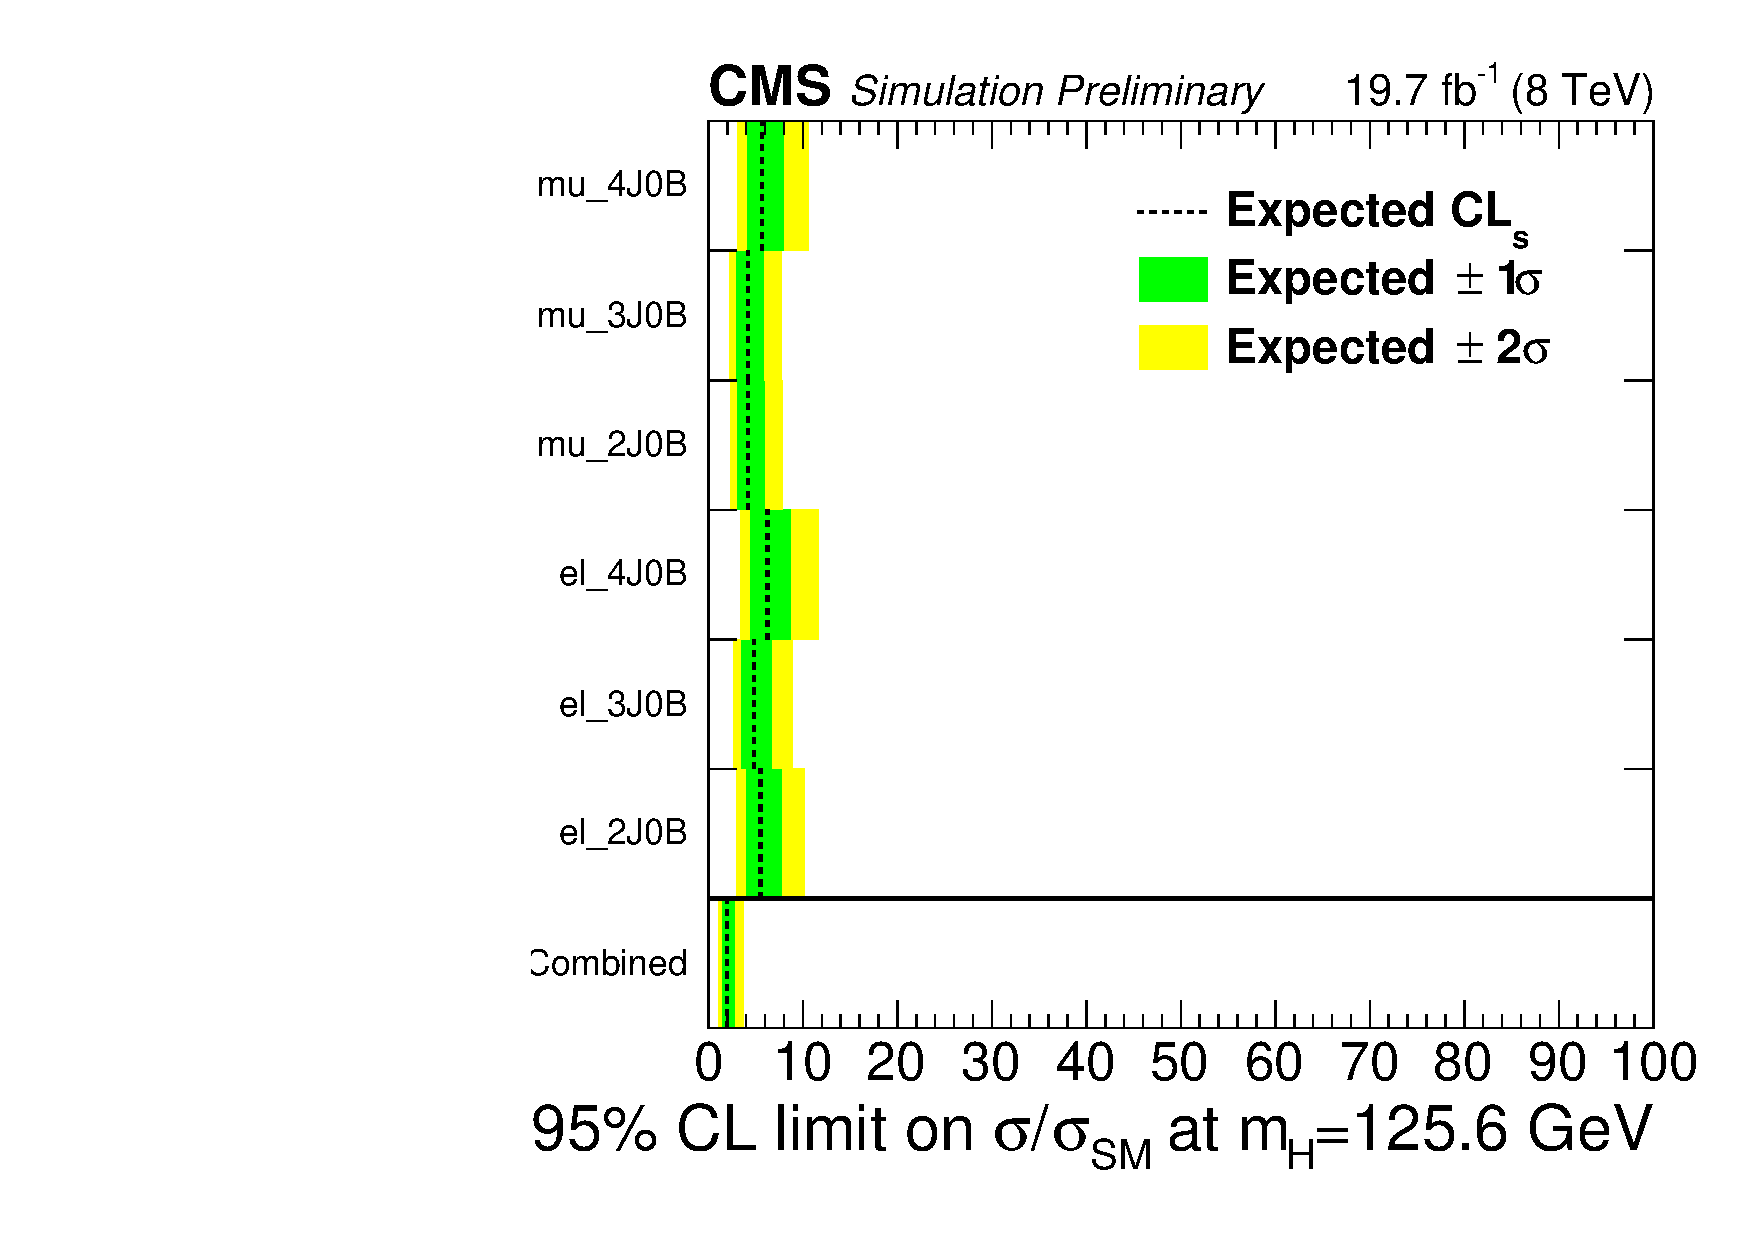
\includegraphics[width=\textwidth]{\figpath/Chapter4/2015_08_01_combinedSM_KinMEBDT_StatsOnly.pdf}
		\label{fig:limits_stats_only}
	\end{subfigure}
	\begin{subfigure}[t]{0.46\textwidth}
		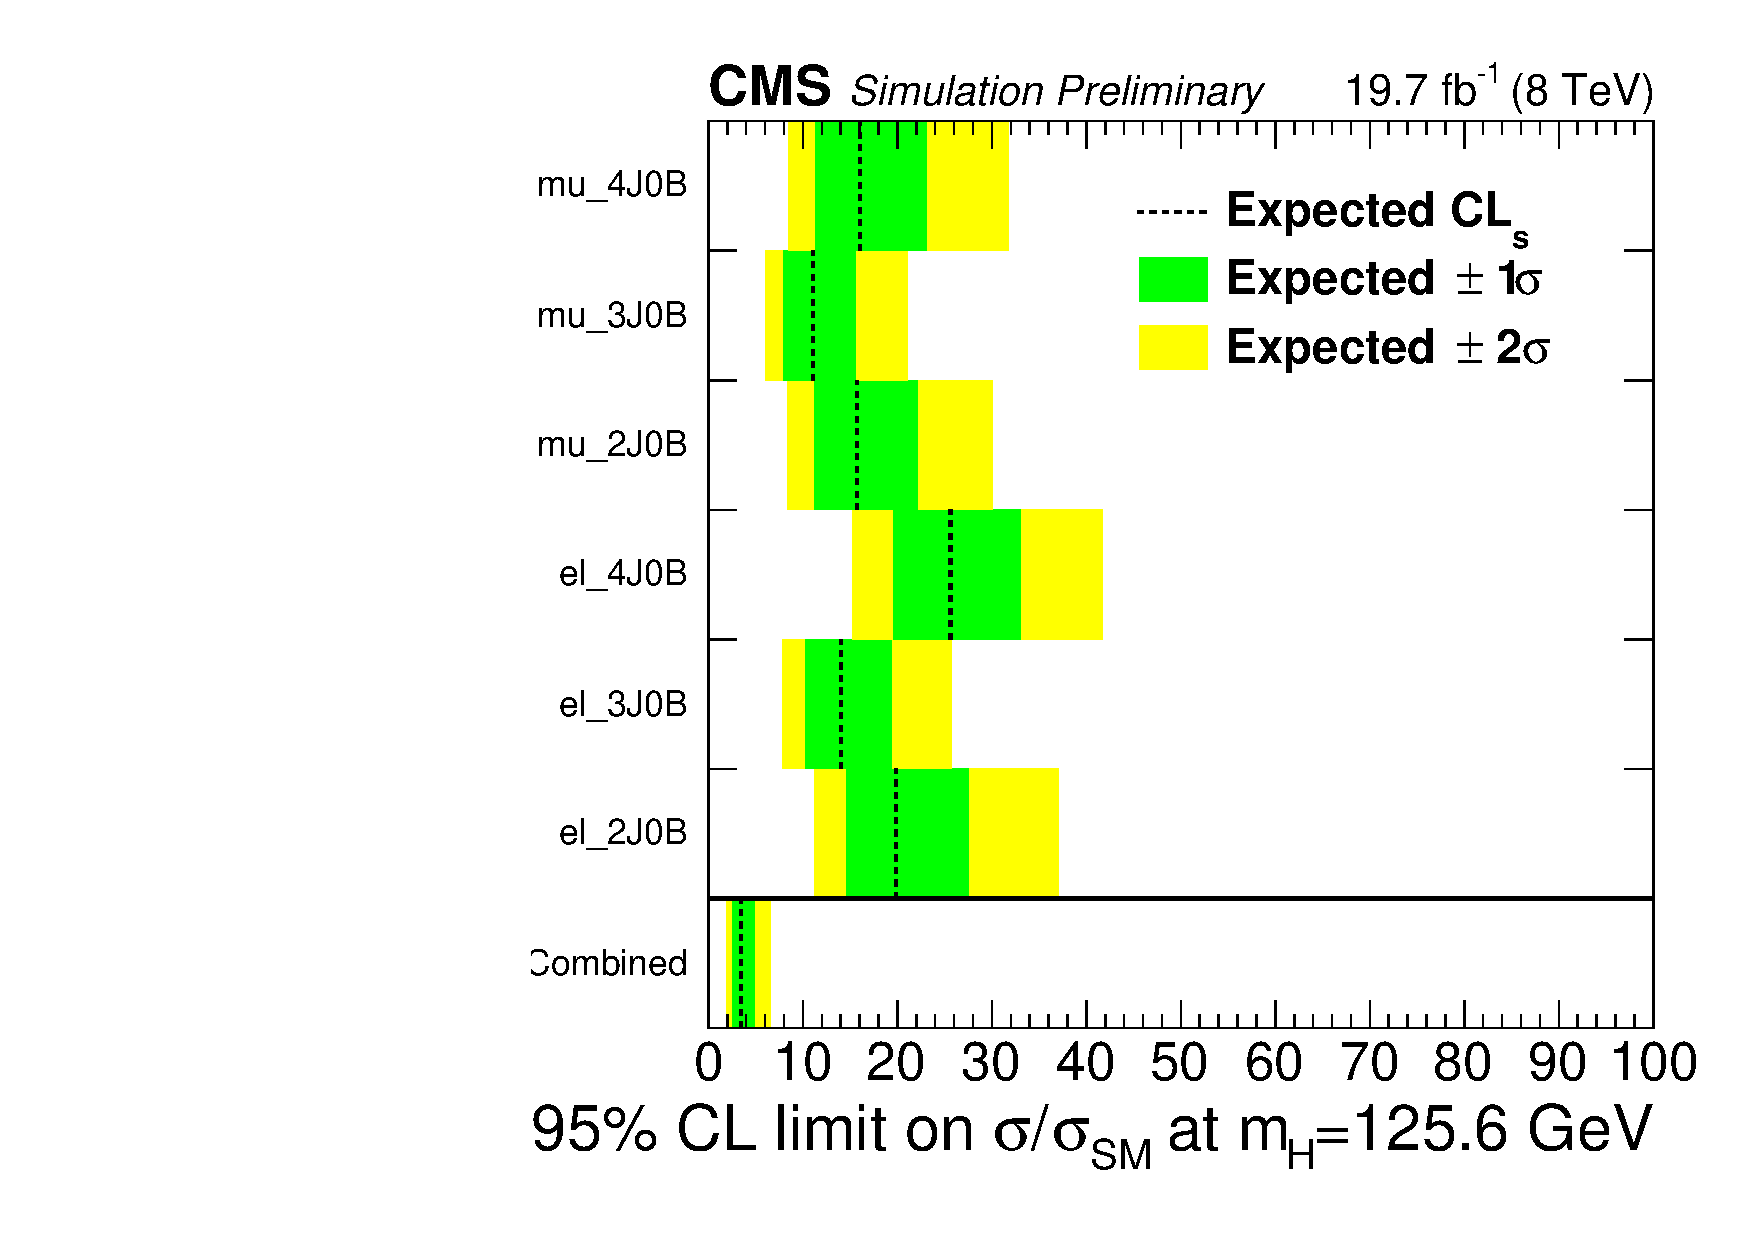
\includegraphics[width=\textwidth]{\figpath/Chapter4/2015_08_01_combinedSM_KinMEBDT.pdf}
		\label{fig:limits_with_sys}
	\end{subfigure}
	\caption{Expected 95\% upper confidence level on the Higgs signal strength (left) without including systematic uncertainties and (right) with systematic uncertainties included. The median combined limit is found to be 2.01 without systematics and 3.48 with them.}
	\label{fig:limits}
\end{figure}
\end{comment}